\subsection{Misura finale}\label{par:fondo2}

\subsubsection{Prese dati}

\begin{table}
	\centering
	\begin{tabular}{lllll}
		Data & Durata & Calibrazioni & Dati & Angolo \\
		\hline
		19--20 feb    & 20 ore & dopo, limitata & istogramma &           45.0\,\si{\degree} \\
		20--22 feb    & 40 ore & dopo           & istogramma &   61$\sfrac34$\,\si{\degree} \\
		26--27 feb    & 22 ore & prima e dopo   & campioni   &           15.0\,\si{\degree} \\
		27 feb--1 mar & 38 ore & prima          & campioni   & \phantom{1}7.0\,\si{\degree}   
	\end{tabular}
	\caption{\label{tab:misure}
	Prese dati per ricavare la massa dell'elettrone.}
\end{table}

Per ricavare la massa dell'elettrone usiamo quattro misure di spettro in coincidenza.
Tutte le misure durano circa 24 ore per avere sufficiente statistica (si è poi rivelata eccessiva).
Era nelle nostre intenzioni avere una calibrazione prima e dopo ogni misura
e avere l'elenco dei campioni anziché solo l'istogramma,
ma la rottura dell'alimentatore del crate ha ostacolato i nostri piani.
La misura dopo la quale il crate si è rotto ha la calibrazione solo prima;
due misure che abbiamo recuperato e che inizialmente erano solo misure di prova hanno la calibrazione solo dopo,
una delle quali non era intesa come misura di calibrazione e quindi ha solo il cobalto
(calibrazione 20feb in \autoref{tab:calibration}).
L'elenco delle misure è riportato in \autoref{tab:misure}.

\subsubsection{Funzione empirica spalla Compton}

\begin{figure}
	\centering
	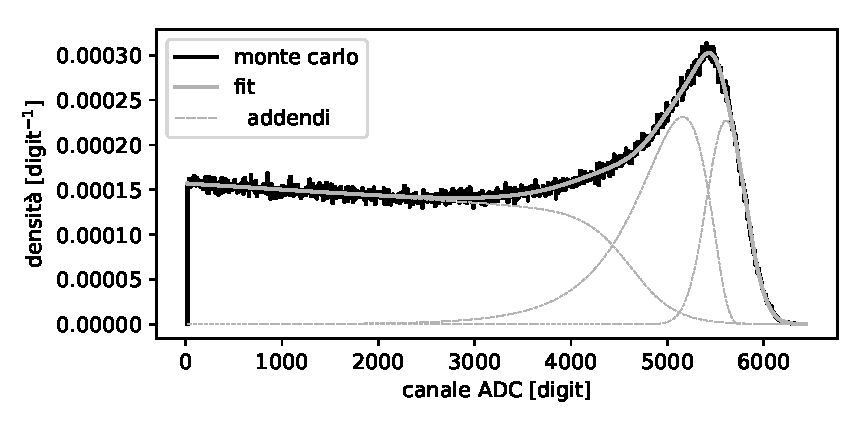
\includegraphics[width=33em]{empirical-secondary}
	\caption{\label{fig:empirical-secondary}
	Funzione empirica per descrivere la spalla Compton,
	ricavata con un fit della somma di una gaussiana, una log-gaussiana e la funzione di Fermi.
	Il monte carlo mostrato è ad angolo \SI{15}{\degree} e fotone della sorgente di \SI{1.33}{MeV}.}
\end{figure}

\begin{figure}
	\centering
	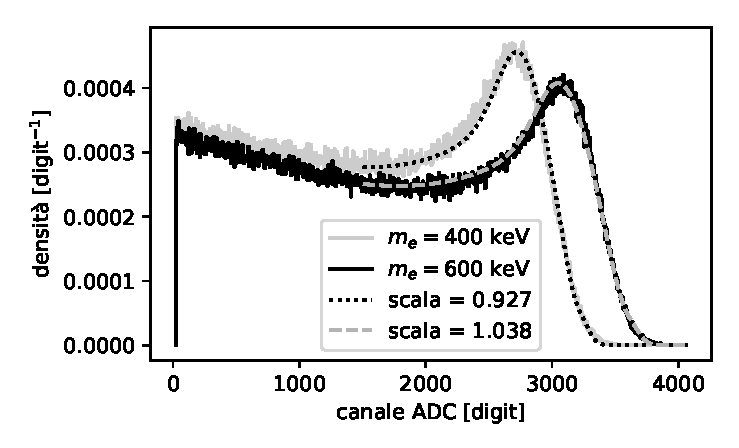
\includegraphics[width=28em]{empirical-test}
	\caption{\label{fig:empirical-test}
	Simulazione della spalla Compton a \SI{45}{\degree} e fotone della sorgente a \SI{1.33}{MeV}
	con diversi valori della massa dell'elettrone,
	fittata con la funzione empirica con solo un parametro di scala libero.}
\end{figure}

Per fare il fit della spalla Compton,
la simuliamo e fittiamo sulla simulazione una funzione empirica a 10 parametri
(vedi \autoref{fig:empirical-secondary});
per usarla sui dati blocchiamo tutti i parametri tranne un parametro di scala.
In \autoref{fig:empirical-test} verifichiamo che,
per valori della massa dell'elettrone di \SI{0.4}{MeV} e \SI{0.6}{MeV},
la funzione descrive ancora sufficientemente bene la curva simulata.
